\documentclass[../Article_Sensitivity_Analsysis.tex]{subfiles}
\graphicspath{{\subfix{../Figures/}}}
\begin{document}
	
	\subsection{Pressure}
	
	As discussed in Chapter \ref{CH:Governing_equations_chapter}, a small pressure wave propagates at the speed of sound relative to the flow. If the flow velocity is relatively low, all pressure changes are hydrodynamic (resulting from velocity motion) rather than thermodynamic. The Low Mach-number assumption leads to instant propagation of the thermodynamic pressure throughout the system. A single pressure value can be considered for the entire system, as all changes occur simultaneously throughout the device. A step-function shown on Figure \ref{fig:Sensitivty_P_P} illustrates the pressure change.
	
	\begin{figure}[h!]
		\centering
		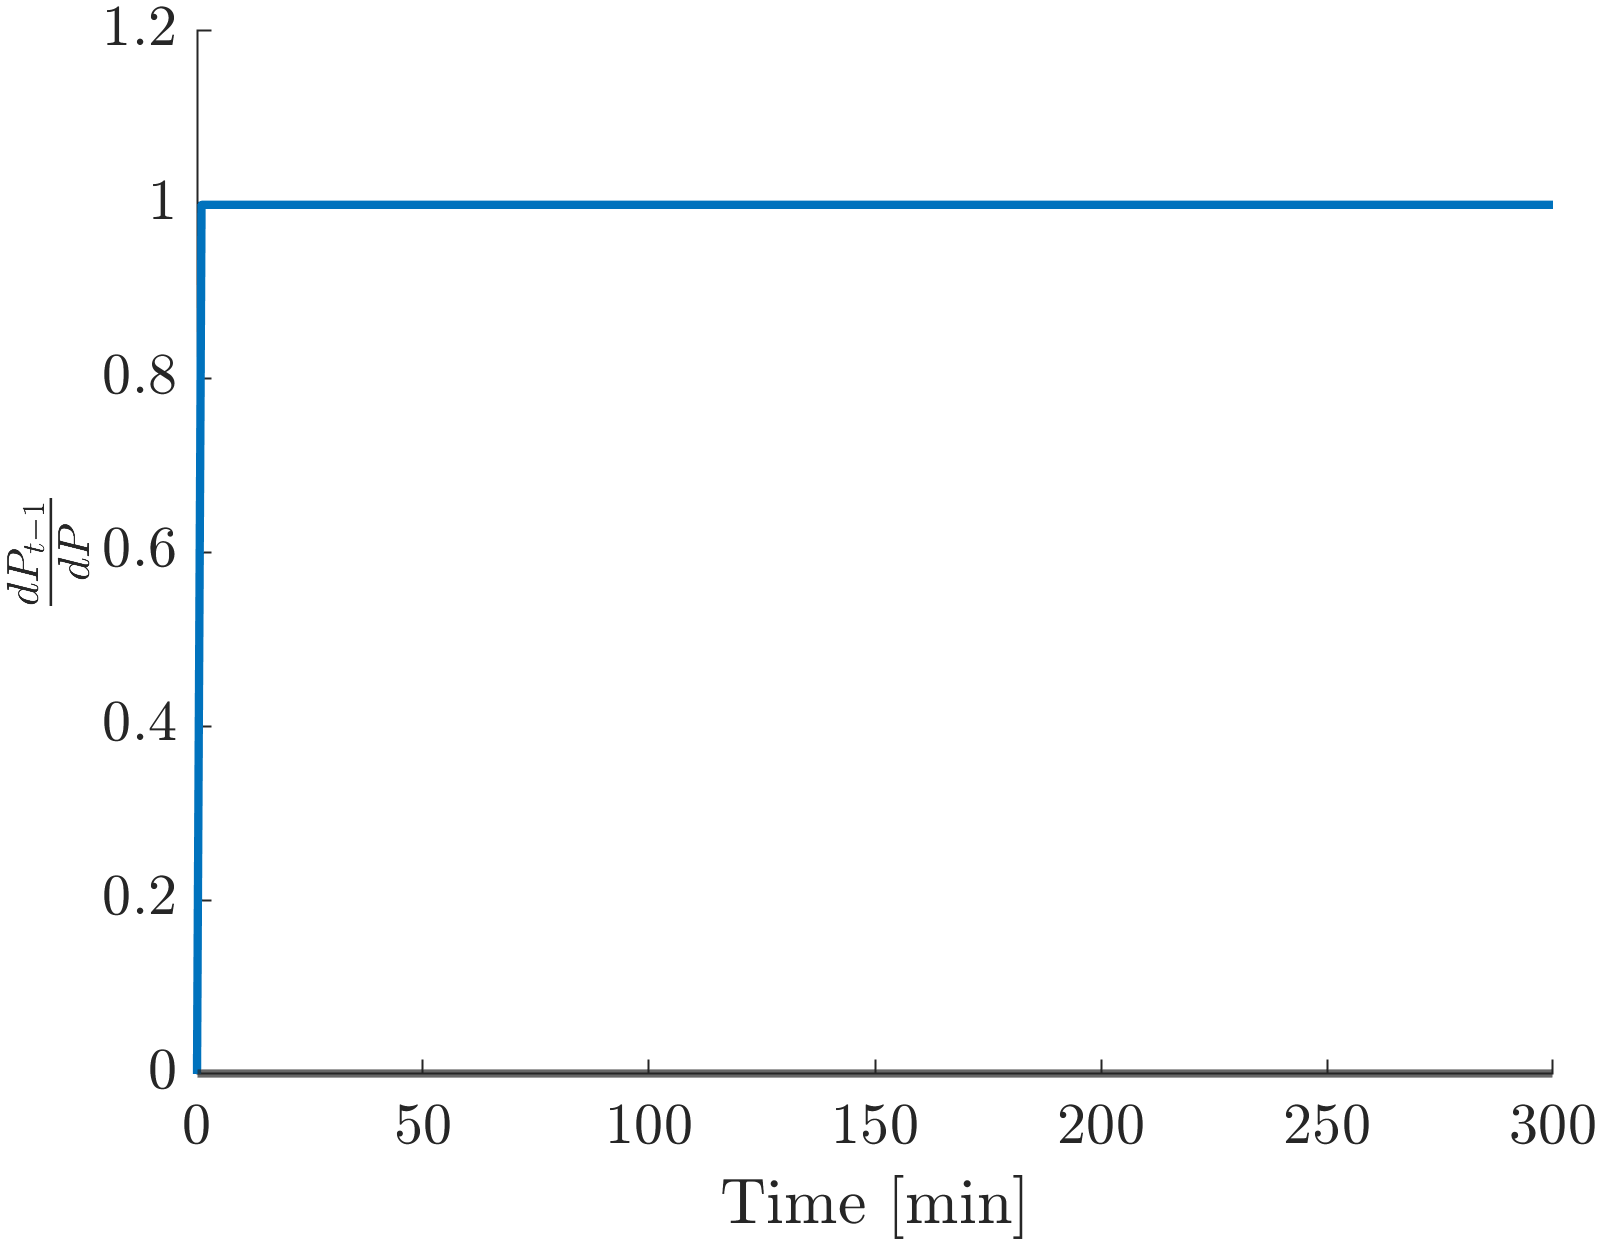
\includegraphics[trim = 0.0cm 0.0cm 0.0cm 0.0cm,clip,width=0.9\columnwidth]{/Results_sensitivity/P_P.png}
		\caption{The effect of $P$ change on $P$ in the system}
		\label{fig:Sensitivty_P_P}
	\end{figure}
	
	\todo{caption and label}
	
	According to Equation \ref{EQ:Enthalpy_equation}, the pressure change directly affects the quantity $h \times \rho$ through $\frac{\partial (P(t) A_f)}{\partial t}$, leading to the step change along the whole system, as presented in Figure \ref{fig:Sensitivty_P_H}. The uniform response across the entire extraction column length and time, represented by the homogeneously dark red colour, indicates that the entire system experiences an immediate and uniform change in enthalpy density in response to pressure changes. 
	
	The pressure change affects the fluid's temperature inside the computational domain, but boundary values are subject to constraints specified at the extremes of that domain. Applying the Dirichlet boundary conditions assumes a fixed temperature value at the inlet, which can lead to a thermal gradient propagating along the system. In contrast, Neumann boundary conditions would dictate the heat flux at the boundaries. In this work, the Neumann boundary conditions equal to zero have been applied, which leads to a uniform response and ensures that the temperatures at the inlet, the outlet, and the middle of the extractor are the same.
	
	\begin{figure}[h!]
		\centering
		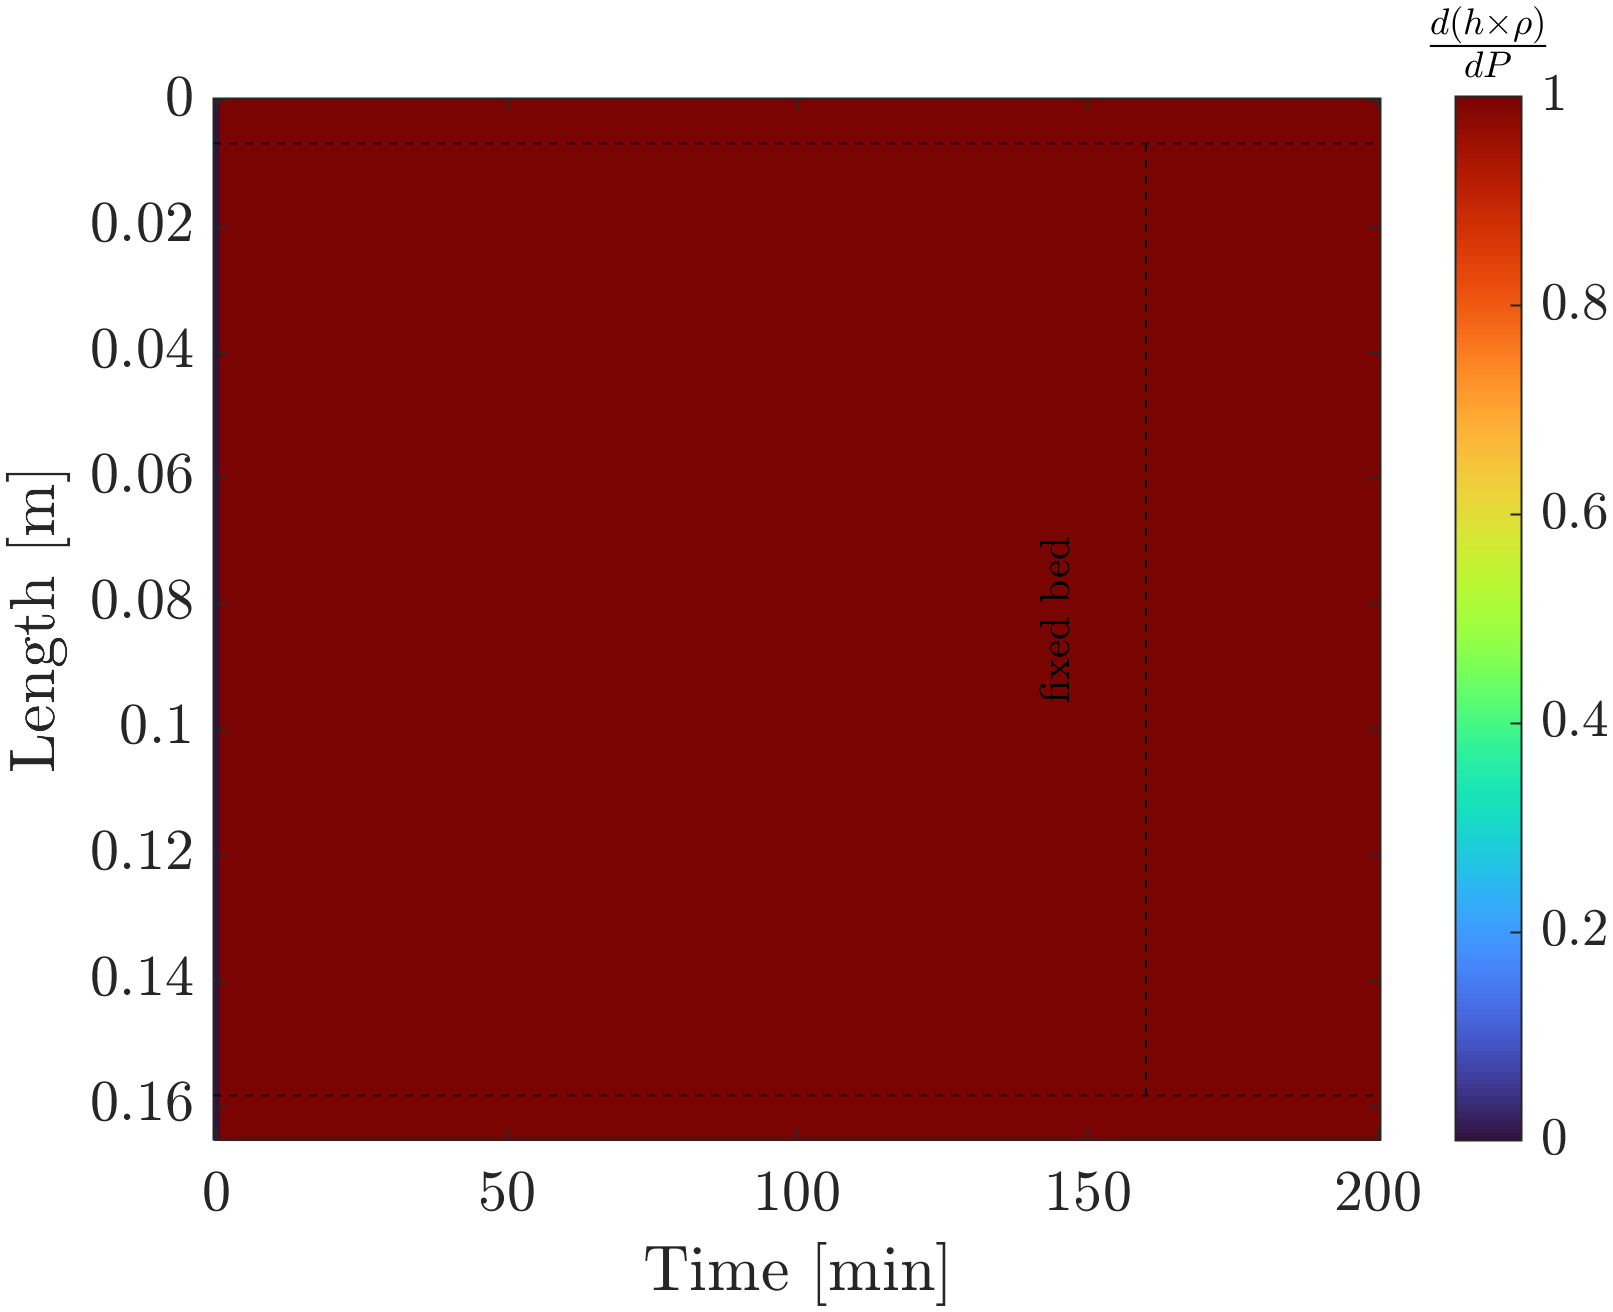
\includegraphics[trim = 0.0cm 0.0cm 0.0cm 0.0cm,clip,width=0.9\columnwidth]{/Results_sensitivity/H_P.png}
		\caption{The effect of $P$ change on $(h \times \rho)$ in the system}
		\label{fig:Sensitivty_P_H}
	\end{figure}
	
	Figure \ref{fig:Sensitivty_P_CS} shows the sensitivity of the solute concentration in the solid phase with respect to pressure change along a fixed bed in a supercritical fluid extraction process. As discussed in Chapter \ref{CH: Continuity}, the velocity of a fluid is inversely proportional to its density, which suggests that with higher fluid density, the velocity decreases. This leads to an extended residence time, ergo, a longer interaction between the solute and the solvent. Initially, the extraction process is in the kinetically-controlled regime, where the concentration gradient is high, and the limiting factor is the solute solubility. As discussed in ({\color{red}article 1}), the system is considered to be far from saturation, which can explain the low system response at the beginning of the process. The system response becomes more evident when the concentration gradient diminishes, and the extraction moves from the kinetic-controlled to the diffusion-controlled regime. The negative sign can be interpreted as a faster loss of a solute from the solid phase, which corresponds to enhanced mass transfer. Over time, the amount of solute becomes a limiting factor, and the pressure change has a lower effect on the system, increasing the negative sensitivities. Eventually, sensitivities approach zero asymptotically. The solute concentration in the solid phase has been reduced, and further changes in pressure have a low influence on the state space.

	\begin{figure}[h!]
		\centering
		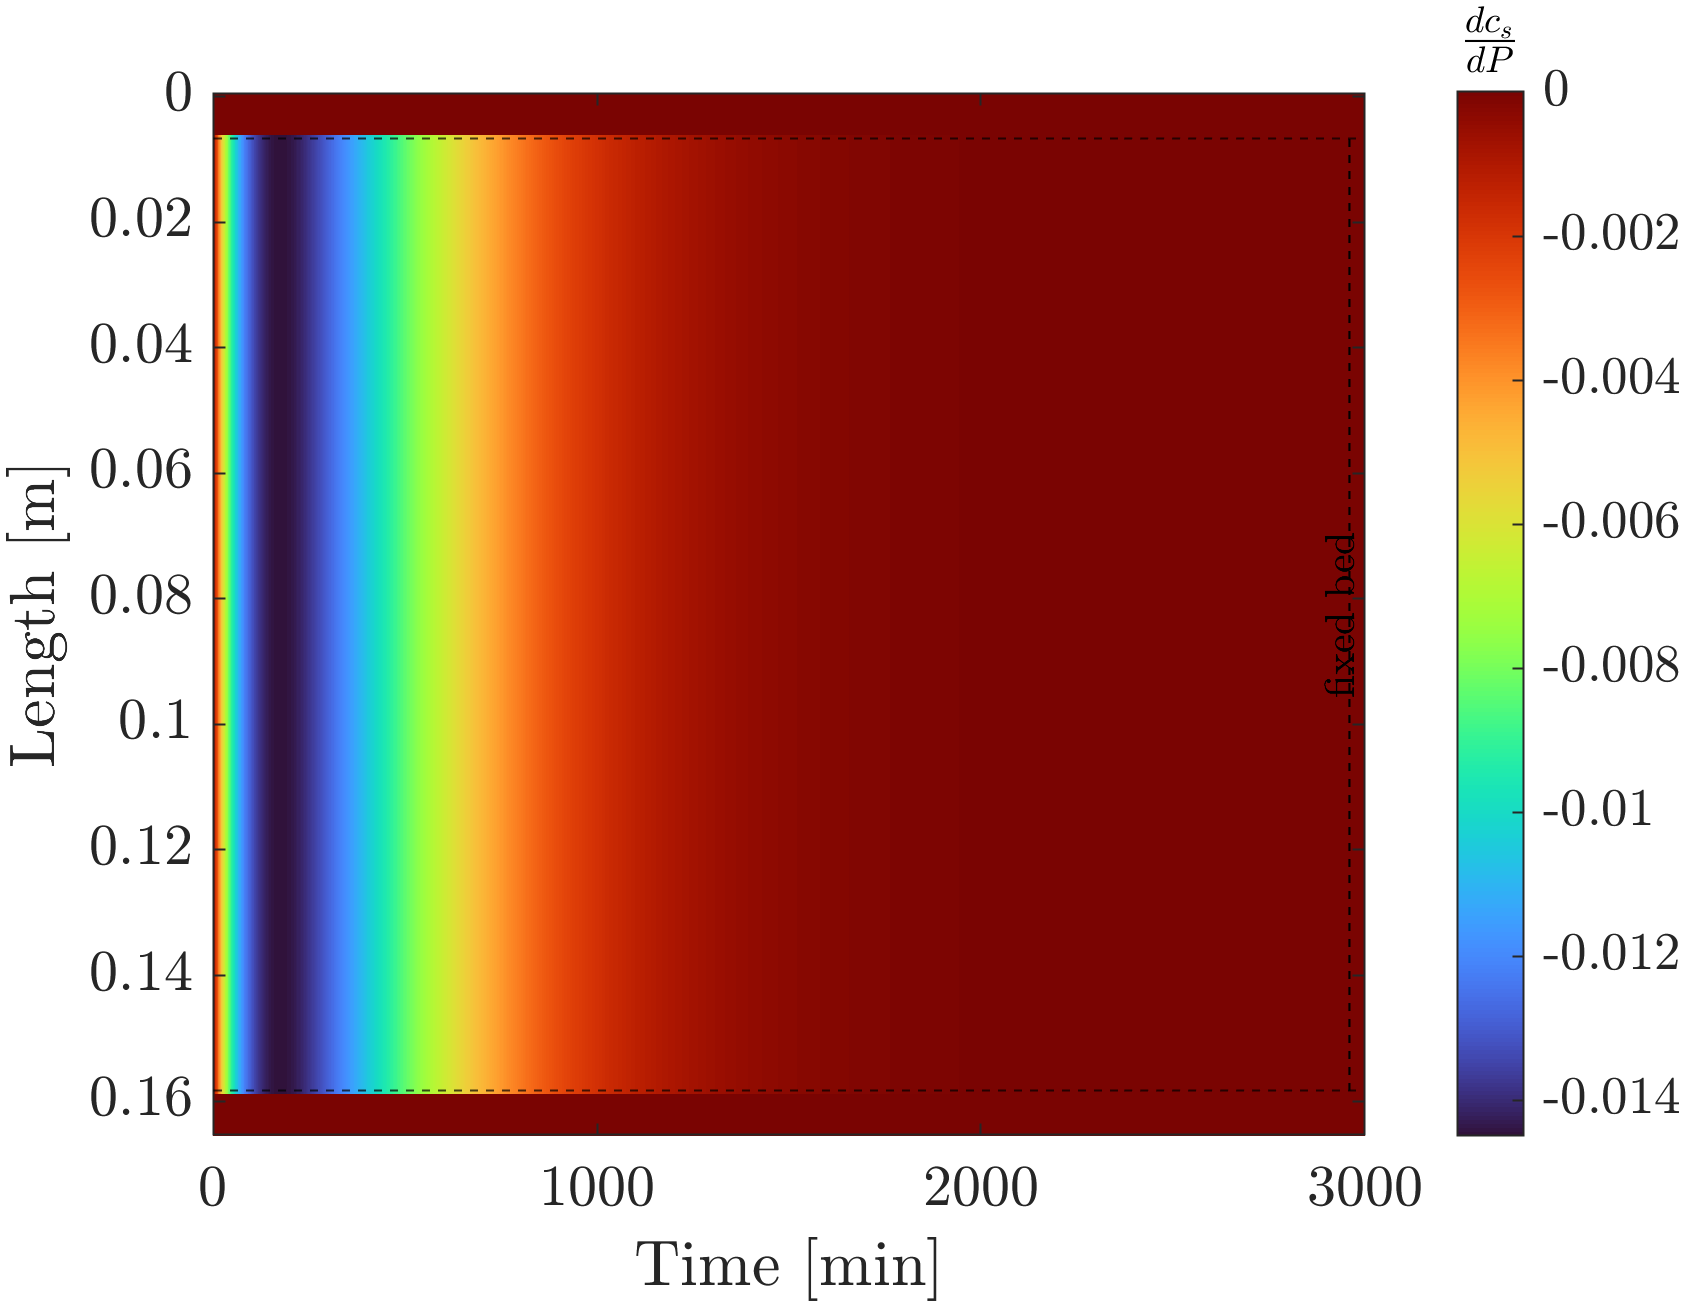
\includegraphics[trim = 0.0cm 0.0cm 0.0cm 0.0cm,clip,width=0.9\columnwidth]{/Results_sensitivity/CS_P.png}
		\caption{The effect of $P$ change on $C_s$}
		\label{fig:Sensitivty_P_CS}
	\end{figure}
	
	Figure \ref{fig:Sensitivty_P_CF} shows the sensitivity of the solute concentration in the fluid phase with respect to the pressure change. As analysed above, an increase in pressure enhances the mass transfer, resulting in the concentration front moving through the system. The system response is initially low, reflecting the idle period discussed above. Later, the sensitivities start to increase due to faster solute loss from the solid phase, which indicates that more solute is transported to the fluid phase. When the amount of solute in the solid phase becomes a limiting factor, the extraction rate slows down, sensitivities decline asymptotic towards zero, and the impact of the pressure change gradually decreases. As the fluid phase is mobile, the advection affects the sensitivities, which causes the sensitivities to move along the system analogously to the solute in the fluid phase.
	
	\begin{figure}[h!]
		\centering
		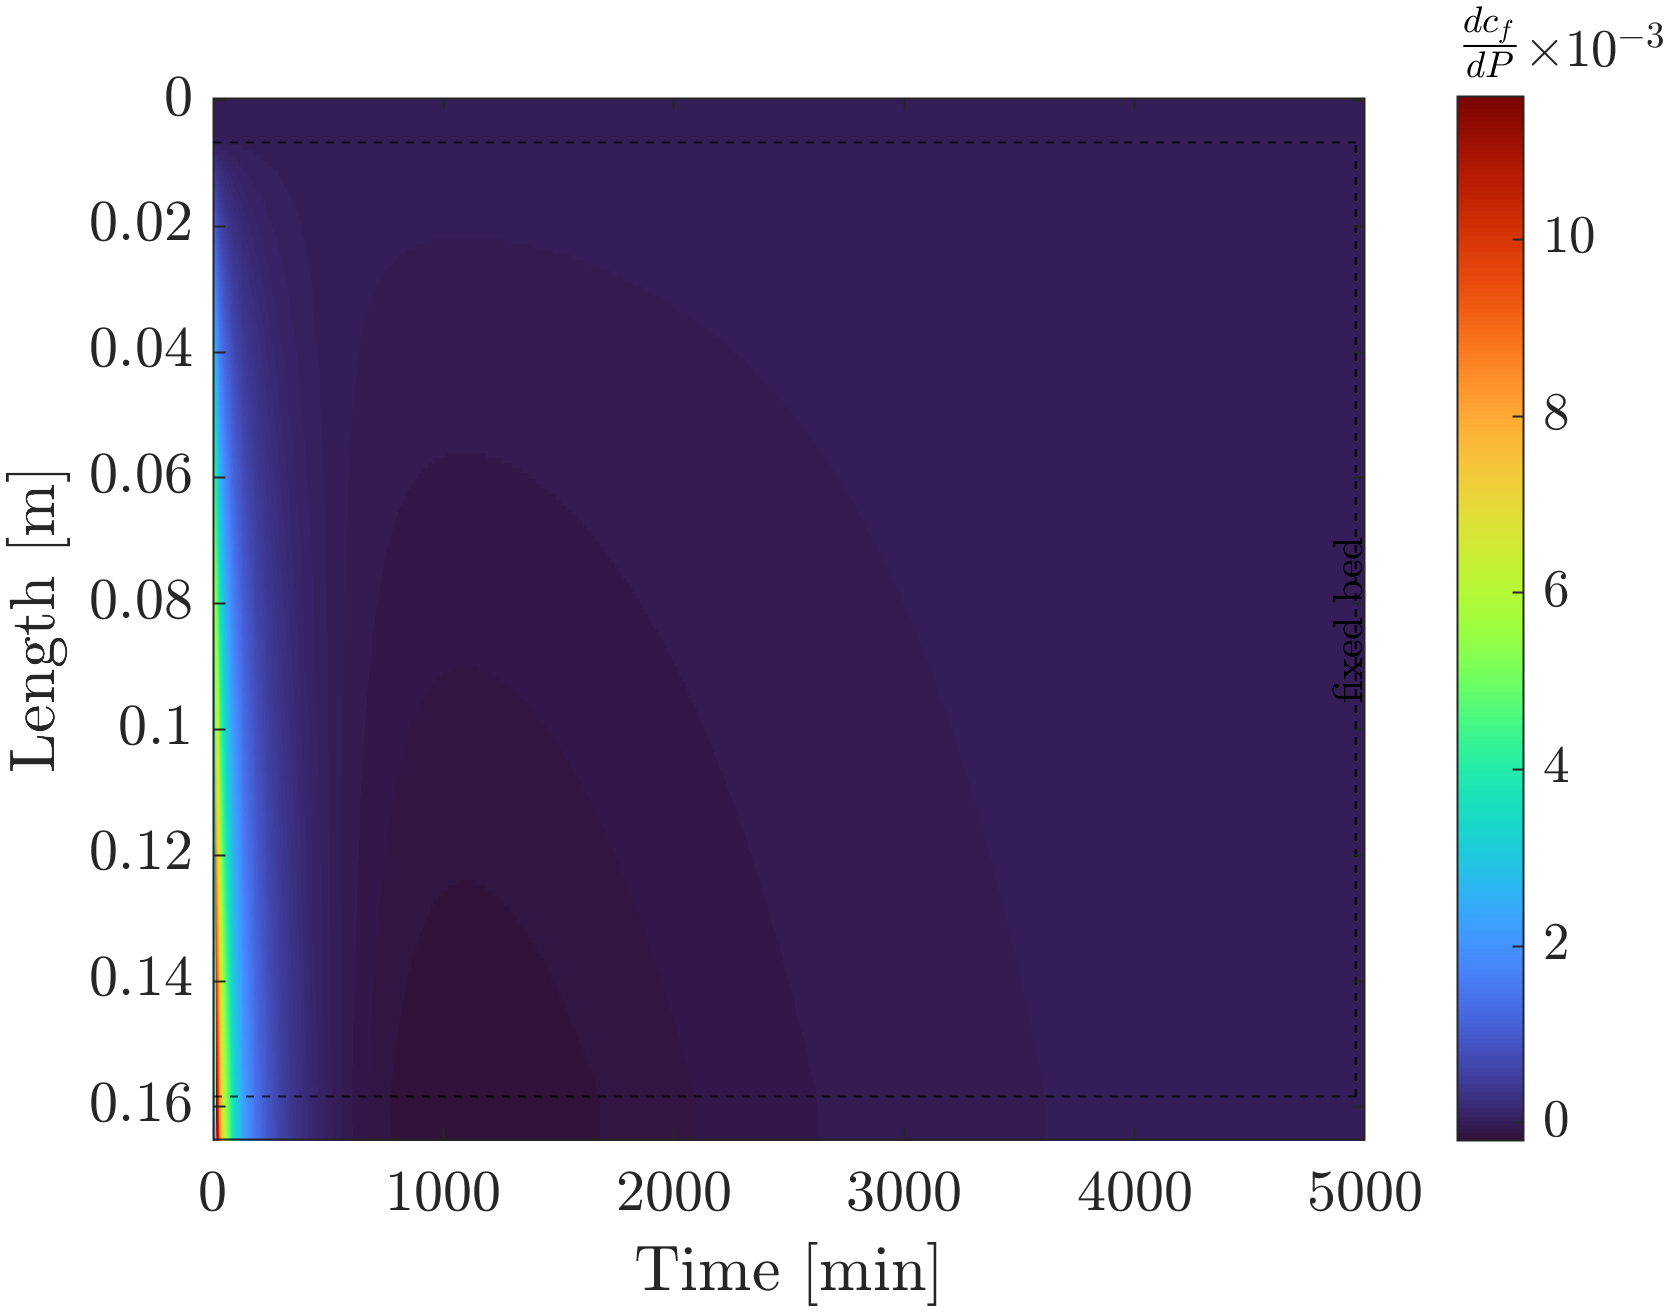
\includegraphics[trim = 0.0cm 0.0cm 0.0cm 0.0cm,clip,width=0.9\columnwidth]{/Results_sensitivity/CF_P.png}
		\caption{The effect of $P$ change on $C_f$}
		\label{fig:Sensitivty_P_CF}
	\end{figure}
	
	Figure \ref{fig:Sensitivty_P_y} illustrates how sensitive the extraction yield is to the pressure change. Initially, the sensitivity curve stays almost flat, suggesting a latency in the system's response to pressure changes. Due to the decreased velocity of the fluid, the solute reaches the extractor's outlet later, which causes minor negative sensitivities to appear. The process continues, and the sensitivity curve increases rapidly when the solute reaches the extractor's outlet. The positive yield sensitivity indicates an improvement in the process efficiency, which is directly related to enhanced mass transfer. The peak in $\frac{dy}{dP}$ reflects when the deviation from the original system is the largest. Beyond the peak, the sensitivity declines and converges towards zero. The concentration gradient becomes a limiting factor, and the enhanced mass transfer no longer plays a dominant role compared to the original system.
	
	\begin{figure}[h!]
		\centering
		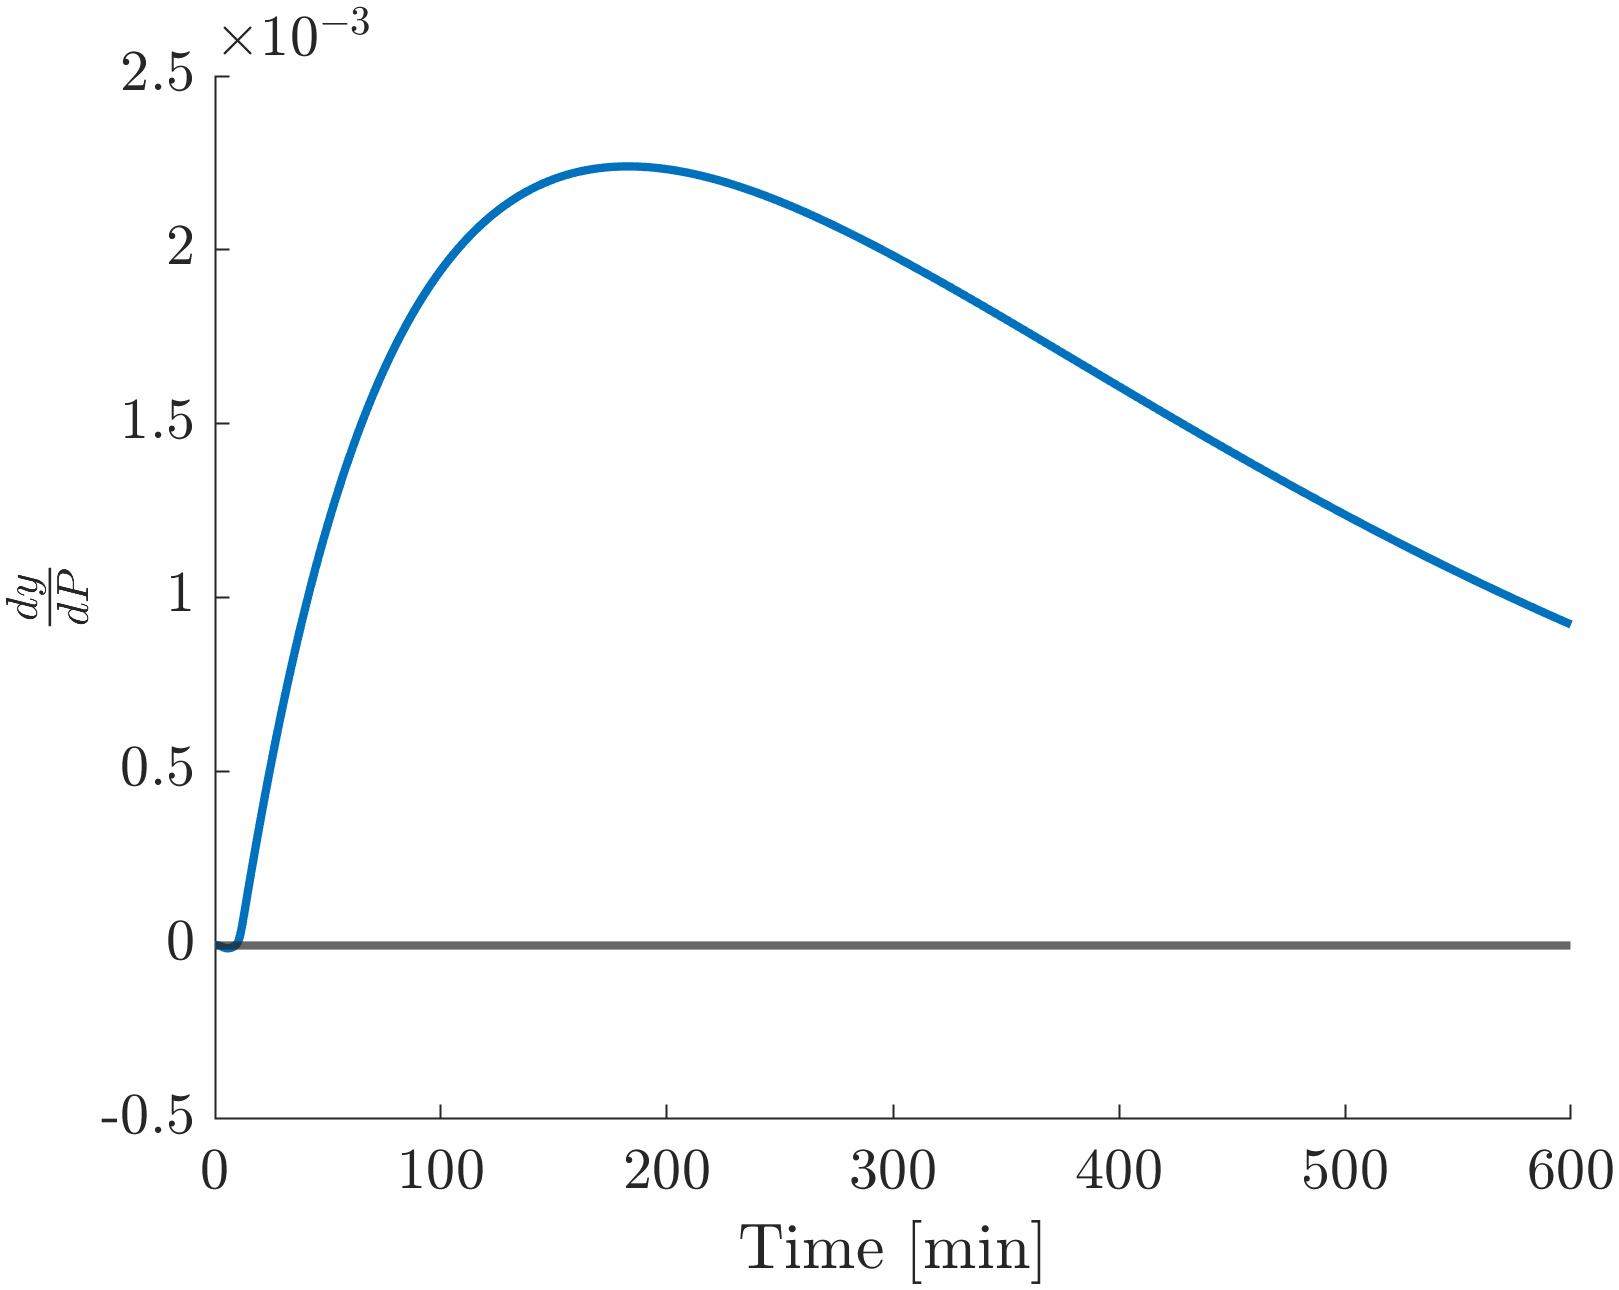
\includegraphics[trim = 0.0cm 0.0cm 0.0cm 0.0cm,clip,width=0.9\columnwidth]{/Results_sensitivity/Y_P.png}
		\caption{The effect of $P$ change on $y(t)$}
		\label{fig:Sensitivty_P_y}
	\end{figure}
		
\end{document}


































